\documentclass{article}

\usepackage{amsmath,amssymb}
\usepackage{tikz}
\usepackage{pgfplots}
\usepackage{xcolor}
\usepackage[left=2.1cm,right=3.1cm,bottom=3cm,footskip=0.75cm,headsep=0.5cm]{geometry}
\usepackage{enumerate}
\usepackage{enumitem}
\usepackage{marvosym}
\usepackage{tabularx}
\usepackage{multirow}
\usepackage[colorlinks = true, linkcolor = blue, urlcolor  = blue, citecolor = blue, anchorcolor = blue]{hyperref}

\usepackage{listings}
\definecolor{lightlightgray}{rgb}{0.95,0.95,0.95}
\definecolor{lila}{rgb}{0.8,0,0.8}
\definecolor{mygray}{rgb}{0.5,0.5,0.5}
\definecolor{mygreen}{rgb}{0,0.8,0.26}
\lstdefinestyle{java} {language=java}
\lstset{language=java,
	basicstyle=\ttfamily,
	keywordstyle=\color{lila},
	commentstyle=\color{lightgray},
	stringstyle=\color{mygreen}\ttfamily,
	backgroundcolor=\color{white},
	showstringspaces=false,
	numbers=left,
	numbersep=10pt,
	numberstyle=\color{mygray}\ttfamily,
	identifierstyle=\color{blue},
	xleftmargin=.1\textwidth, 
	%xrightmargin=.1\textwidth,
	escapechar=§,
}

\usepackage[utf8]{inputenc}

\renewcommand*{\arraystretch}{1.4}

\newcolumntype{L}[1]{>{\raggedright\arraybackslash}p{#1}}
\newcolumntype{R}[1]{>{\raggedleft\arraybackslash}p{#1}}
\newcolumntype{C}[1]{>{\centering\let\newline\\\arraybackslash\hspace{0pt}}m{#1}}

\newcommand{\E}{\mathbb{E}}
\DeclareMathOperator{\rk}{rk}
\DeclareMathOperator{\Var}{Var}
\DeclareMathOperator{\Cov}{Cov}
\DeclareMathOperator{\SD}{SD}
\DeclareMathOperator{\Cor}{Cor}

\title{\textbf{Instrumente des Finanzmanagements, Tutorium 2}}
\author{\textsc{Henry Haustein}}
\date{}

\begin{document}
	\maketitle
	
	\section*{Aufgabe 2K279: Kapitalmarkt- und Portfoliotheorie}
	\begin{enumerate}[label=(\alph*)]
		\item Die Renditen sind
		\begin{align}
			r_M &= 0.15\cdot -0.1 + 0.25\cdot 0.2 + 0.6\cdot 0.15 = 0.125 \notag \\
			r_f &= 0.05 \notag \\
			r_{Win} &= 0.15\cdot -0.05 + 0.25\cdot 0.25 + 0.6\cdot 0.1 = 0.115 \notag \\
			r_{Bear} &= 0.15\cdot 0.3 + 0.25\cdot -0.05 + 0.6\cdot 0.15 = 0.1225 \notag
		\end{align}
		Die Standardabweichungen sind
		\begin{align}
			\SD(r_M) &= \sqrt{0.15(-0.1-0.125)^2 + 0.25(0.2-0.125)^2 + 0.6(0.15-0.125)^2} = 0.0968 \notag \\
			\SD(r_f) &= 0 \notag \\
			\SD(r_{Win}) &= \sqrt{0.15(-0.05-0.115)^2 + 0.25(0.25-0.115)^2 + 0.6(0.1-0.115)^2} = 0.0937 \notag \\
			\SD(r_M) &= \sqrt{0.15(0.3-0.1225)^2 + 0.25(-0.05-0.1225)^2 + 0.6(0.15-0.1225)^2} = 0.1123 \notag
		\end{align}
		Die Covarianzen sind
		\begin{align}
			\Cov(r_M,r_M) &= \SD(r_M)^2 = 0.0968^2 = 0.00937024 \notag \\
			\Cov(r_f,r_M) &= 0 \notag \\
			\Cov(r_{Win},r_M) &= 0.15(-0.05-0.115)(-0.1-0.125) + 0.25(0.25-0.115)(0.2-0.125) \notag \\
			&+ 0.6(0.1-0.115)(0.15-0.125) = \frac{63}{8000} \notag \\
			\Cov(r_{Bear},r_M) &= 0.15(0.3-0.1225)(-0.1-0.125) + 0.25(-0.05-0.1225)(0.2-0.125) \notag \\
			&+ 0.6(0.15-0.1225)(0.15-0.125) = -\frac{141}{16000} \notag
		\end{align}
		Die Betas sind
		\begin{align}
			\beta_M &= \frac{\Cov(r_M,r_M)}{\SD(r_M)^2} = \frac{0.00937024}{0.00937024} = 1 \notag \\
			\beta_f &= \frac{\Cov(r_f,r_M)}{\SD(r_M)^2} = \frac{0}{0.00937024} = 0 \notag \\
			\beta_{Win} &= \frac{\Cov(r_f,r_M)}{\SD(r_M)^2} = \frac{63}{8000\cdot 0.00937024} = 0.8404 \notag \\
			\beta_{Bear} &= \frac{\Cov(r_f,r_M)}{\SD(r_M)^2} = -\frac{141}{16000\cdot 0.00937024} = -0.9391 \notag
		\end{align}
		Kapitalmarktkennlinie und Wertpapierkennlinie:
		\begin{center}
			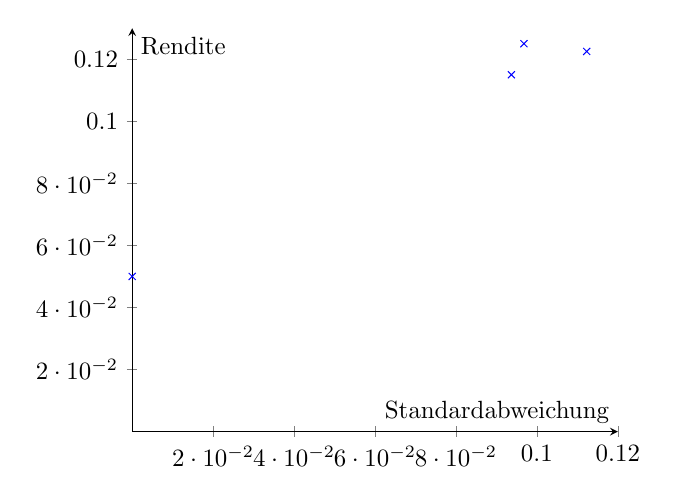
\begin{tikzpicture}[scale=0.9]
				\begin{axis}[
					xmin=0, xmax=0.12, xlabel=Standardabweichung,
					ymin=0, ymax=0.13, ylabel=Rendite,
					samples=400,
					axis x line=middle,
					axis y line=middle,
					domain=0:1,
					]
					\addplot[blue, mark=x,only marks] coordinates {
						(0.0968,0.125)
						(0,0.05)
						(0.0937,0.115)
						(0.1123,0.1225)
					};
					
				\end{axis}
			\end{tikzpicture}
			\begin{tikzpicture}
				\begin{axis}[
					xmin=-1, xmax=1, xlabel=$\beta$,
					ymin=0, ymax=0.13, ylabel=Rendite,
					samples=400,
					axis x line=middle,
					axis y line=middle,
					domain=-1:1,
					]
					\addplot[blue, mark=x,only marks] coordinates {
						(1,0.125)
						(0,0.05)
						(0.8404,0.115)
						(-0.9391,0.1225)
					};
					\addplot[red] {0.075*x+0.05};
				\end{axis}
			\end{tikzpicture}
		\end{center}
		\item Marktpreis des Risikos:
		\begin{align}
			\frac{r_M-r_f}{\SD(r_M)} = \frac{0.125-0.05}{0.0968} = 0.7748 \notag
		\end{align}
		\item Beide Aktien liegen über der Wertpapierkennlinie, also sind sie unterbewertet, weil beide zu viel Rendite geben.
		\item Die Korrelationen sind
		\begin{align}
			\Cor(r_{Win},r_{Bear}) &= \frac{\Cov(r_{Win},r_{Bear})}{\SD(r_{Win})\cdot\SD(r_{Bear})} = \frac{-\frac{837}{80000}}{0.0937\cdot 0.1123} = -0.9943 \notag \\
			\Cor(r_{Win},r_M) &= \frac{\Cov(r_{Win},r_M)}{\SD(r_{Win})\cdot\SD(r_M)} = \frac{\frac{63}{8000}}{0.0937\cdot 0.0968} = 0.8682 \notag \\
			\Cor(r_{Bear},r_M) &= \frac{\Cov(r_{Bear},r_M)}{\SD(r_{Bear})\cdot\SD(r_M)} = \frac{-\frac{141}{16000}}{0.1123\cdot 0.0968} = -0.8107 \notag
		\end{align}
		\item Die Anteile im Portfolio sind
		\begin{align}
			x_{Win} &= \frac{\Var(r_{Bear}) - \Cov(r_{Win},r_{Bear})}{\Var(r_{Bear}) + \Var(r_{Win}) - 2\cdot\Cov(r_{Win},r_{Bear})} \notag \\
			&= \frac{0.1123^2+\frac{837}{80000}}{0.1123^2 + 0.0937^2 + 2\cdot\frac{837}{80000}} = 0.5453 \notag \\
			x_{Bear} &= 1-x_{Win} = 0.4547 \notag
		\end{align}
		Damit ist die Rendite und die Standardabweichung des Portfolios
		\begin{align}
			r_P &= 0.5453\cdot 0.115 + 0.4547\cdot 0.125 = 0.1184 \notag \\
			\SD(r_P) &= 0.003\% \notag
		\end{align}
		\item CAPM liefert
		\begin{align}
			r_{Win}^\ast &= 0.05 + 0.8408(0.125-0.05) = 0.1130 \notag \\
			r_{Bear}^\ast &= 0.05 - 0.9391(0.125-0.05) = -0.0204 \notag
		\end{align}
	\end{enumerate}

	\section*{Aufgabe 11.15: Risiko versus Ertrag}
	\begin{enumerate}[label=(\alph*)]
		\item $r=0.5\cdot 0.07 + 0.5\cdot 0.1=0.085$
		\item $\SD(r)=\sqrt{0.5^2\cdot 0.16^2 + 0.5^2\cdot 0.2^2 + 2\cdot 0.5^2\cdot 0.22\cdot 0.16\cdot 0.2} = 0.1411$
	\end{enumerate}

	\section*{Aufgabe 11.16: Risiko versus Ertrag}
	\begin{enumerate}[label=(\alph*)]
		\item keine Änderung
		\item steigen
	\end{enumerate}

	\section*{Aufgabe 11.17: Risiko versus Ertrag}
	Anteile: Short $\frac{-2000}{10000} = -0.2$, Long $\frac{10000 + 2000}{10000} = 1.2$
	\begin{enumerate}[label=(\alph*)]
		\item $r=1.2\cdot 0.07 - 0.2\cdot 0.1=0.064$
		\item $\SD(r)=\sqrt{1.2^2\cdot 0.16^2 + (-0.2)^2\cdot 0.2^2 + 2\cdot 1.2\cdot (-0.2)\cdot 0.22\cdot 0.16\cdot 0.2} = 0.1873$
	\end{enumerate}

	\section*{Aufgabe 11.21: Risiko versus Ertrag}
	Anteile: Short $\frac{-10000}{10000} = -1$, Long $\frac{10000 + 10000}{10000} = 2$
	\begin{enumerate}[label=(\alph*)]
		\item $r=2\cdot 0.15 - 1\cdot 0.12=0.18$
		\item $\SD(r)=\sqrt{2^2\cdot 0.3^2 + (-1)^2\cdot 0.25^2 + 2\cdot 2\cdot (-1)\cdot 0.9\cdot 0.3\cdot 0.25} = 0.3905$
	\end{enumerate}
	
	\section*{Aufgabe 11.34: Die Bestimmung der Risikoprämie}
	\begin{enumerate}[label=(\alph*)]
		\item $\beta = \Cor(r_{JJ},r_M)\cdot\frac{\SD(r_{JJ})}{\SD(r_M)}=0.06\cdot\frac{0.2}{0.16}=0.075$
		\item $r_f+\beta(r_M-r_f)=0.04+0.075(0.1-0.04)=0.0445$
	\end{enumerate}
	
	\section*{Aufgabe 11.35: Die Bestimmung der Risikoprämie}
	\begin{align}
		\beta_P &= 0.6\cdot 2.16 + 0.4\cdot 0.69 = 1.572 \notag \\
		r_P &= 0.04 + 1.572(0.1.-0.04) = 0.1343 \notag
	\end{align}
	
\end{document}